\section{The \pktlanguage compiler backend}
\subsection{Expression flattening to three-address code}
As a first step, we convert code into three-address code, where all
instructions are either reads / writes into stateful variables or carry out
packet manipulations of the form: \texttt{pkt.f1 = pkt.f2 op pkt.f3;} where
\texttt{op} includes all arithmetic, logical, and relational operators. We also
allow either pkt.f2 or pkt.f3 to be an opaque function call of multiple packet
fields, because \pktlanguage assumes opaque functions are supported in
hardware. Three-address code is similar to P4's action primitives
today~\cite{p4spec}.

To generate code three-address code, we flatten expressions that are not
already legal three-address code, by introducing enough temporaries. For
instance, \texttt{pkt.f = pkt.f1 + pkt.f2 - pkt.f3;} would be flattened to
\texttt{pkt.tmp = pkt.f2 - pkt.f3;} followed by \texttt{pkt.f = pkt.f1 +
pkt.tmp;}

\begin{figure}[!h]
\begin{tiny}
\begin{lstlisting}
pkt.id00 = hash2(pkt.sport, pkt.dport) % 8000;
pkt.saved_hop00 = saved_hop[pkt.id00];
pkt.id10 = hash2(pkt.sport, pkt.dport) % 8000;
pkt.last_time00 = last_time[pkt.id10];
pkt.new_hop0 = hash3(pkt.sport, pkt.dport, pkt.arrival_time) % 64;
pkt.tmp1 = pkt.arrival_time - pkt.last_time00;
pkt.tmp00 = pkt.tmp1 > 5;
pkt.saved_hop01 = (pkt.tmp00) ? (pkt.new_hop0) : pkt.saved_hop00;
pkt.last_time01 = pkt.arrival_time;
pkt.next_hop0 = (pkt.tmp00) ? (pkt.new_hop0) : pkt.saved_hop00;
saved_hop[pkt.id00] = (pkt.tmp00) ? (pkt.new_hop0) : pkt.saved_hop00;
last_time[pkt.id10] = pkt.arrival_time;
\end{lstlisting}
\end{tiny}
\caption{Flowlet switching in three-address code}
\label{fig:three_address}
\end{figure}

\subsection{Code partitioning}
At this point, the code is still in sequential form. Code partitioning
turns sequential code into an atom grid that can be run by \absmachine , by
exploiting parallelism within and across pipeline stages.
To partition code, we carry out the following steps:
\begin{enumerate}
  \item Create a node for each statement in the packet transaction after
    expression flattening.
  \item Create a bidrectional edge between N1 and N2 where N1 is a read from a
    state scalar / state array and N2 is a write into the same state scalar /
    state array.
  \item Create an edge (N1, N2) for every pair of nodes N1, N2 where N2 reads
    a variable written by N1.
  \item Generate strongly connected components (SCCs) of the resulting graph (Figure~\ref{fig:deps}) and condense
    the SCCs to to create a directed acyclic graph (DAG) (Figure~\ref{fig:dag}).
  \item Schedule the resulting DAG using critical path
    scheduling~\cite{crit_path_sched}, creating a new pipeline stage everytime
    one operation needs to follow another (Figure~\ref{fig:pipeline}).
\end{enumerate}

\begin{figure*}
  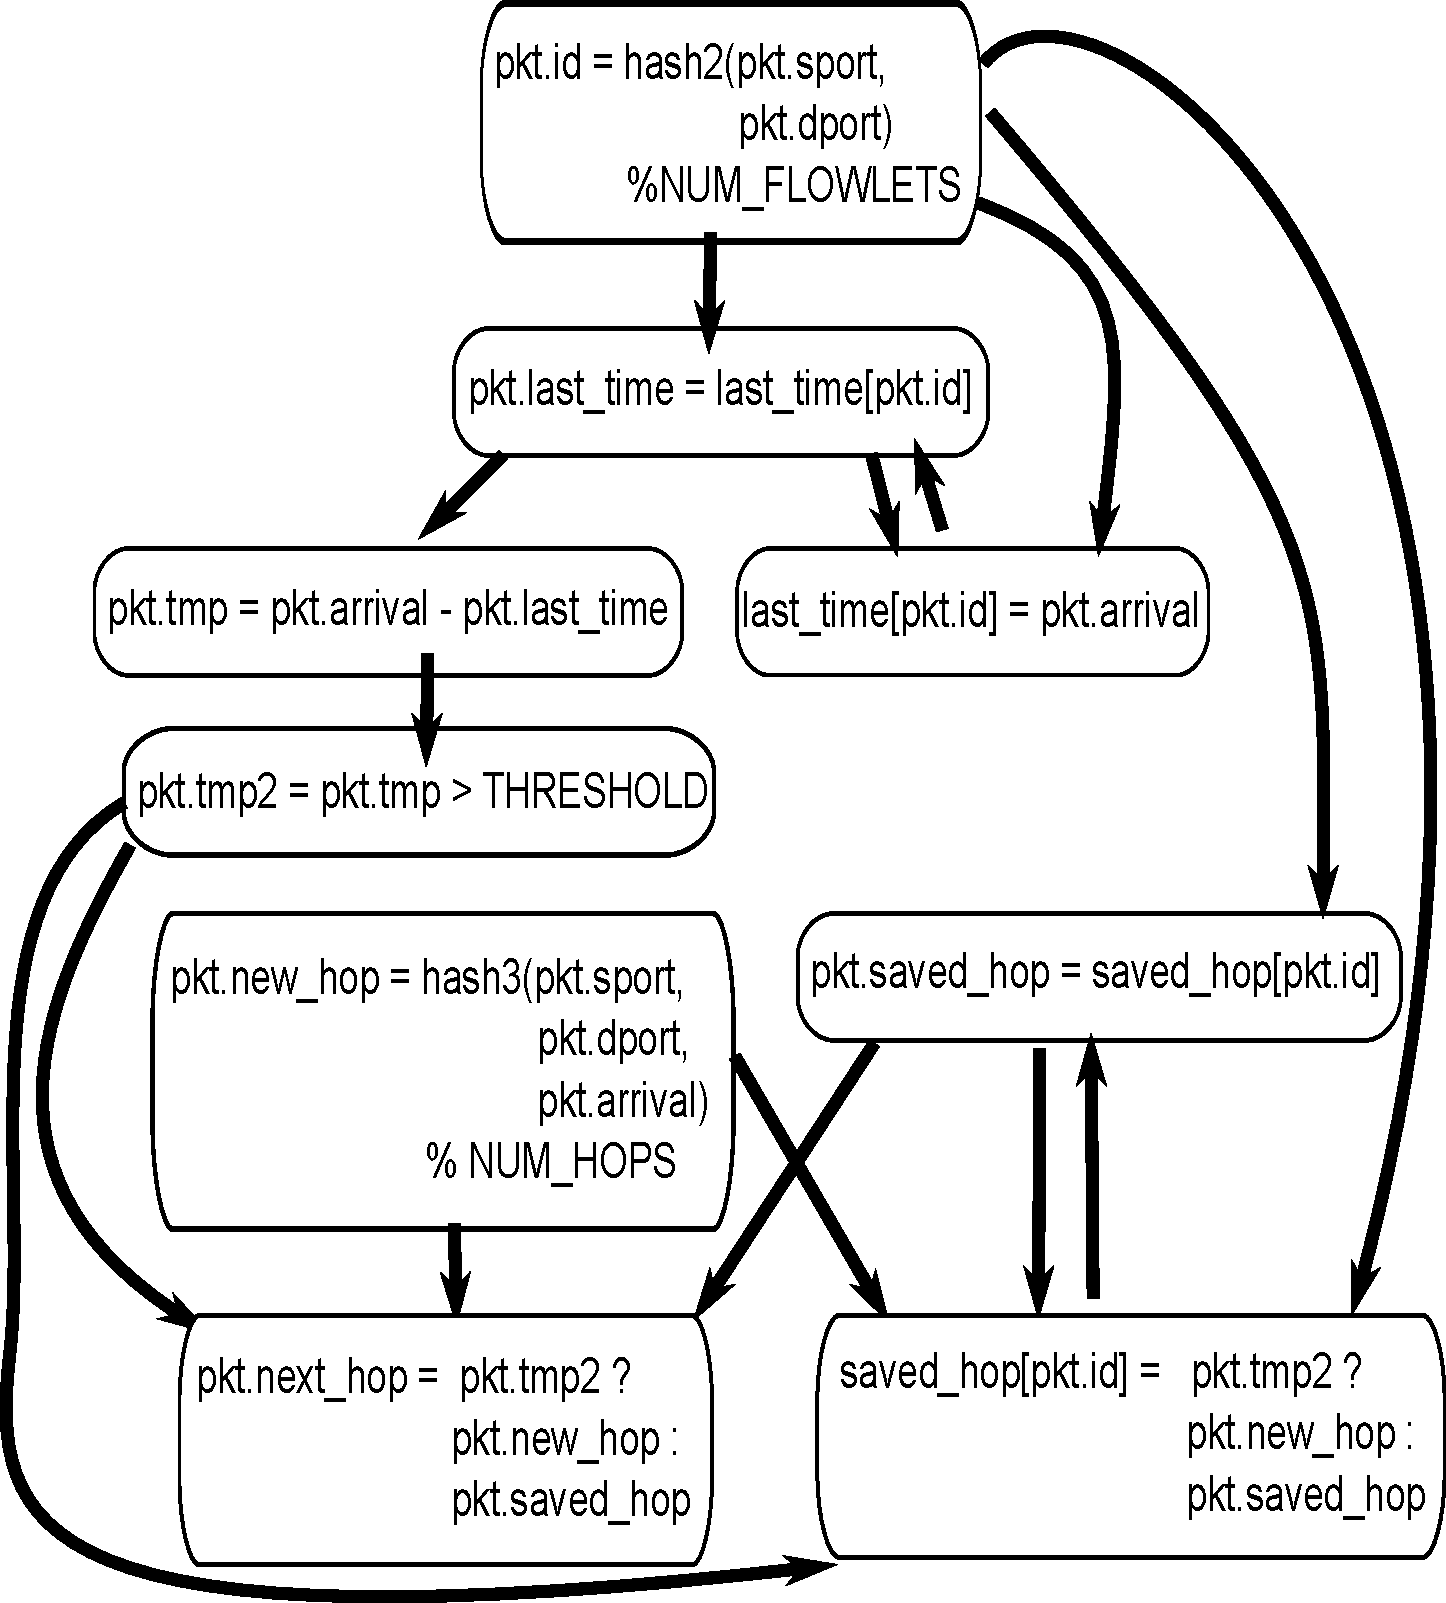
\includegraphics[width=\textwidth]{deps.pdf}
  \caption{Dependency graph of code shown in Figure~\ref{fig:three_address}}
  \label{fig:deps}
\end{figure*}

\subsection{Stateful atoms}

\newpage
\begin{figure}
  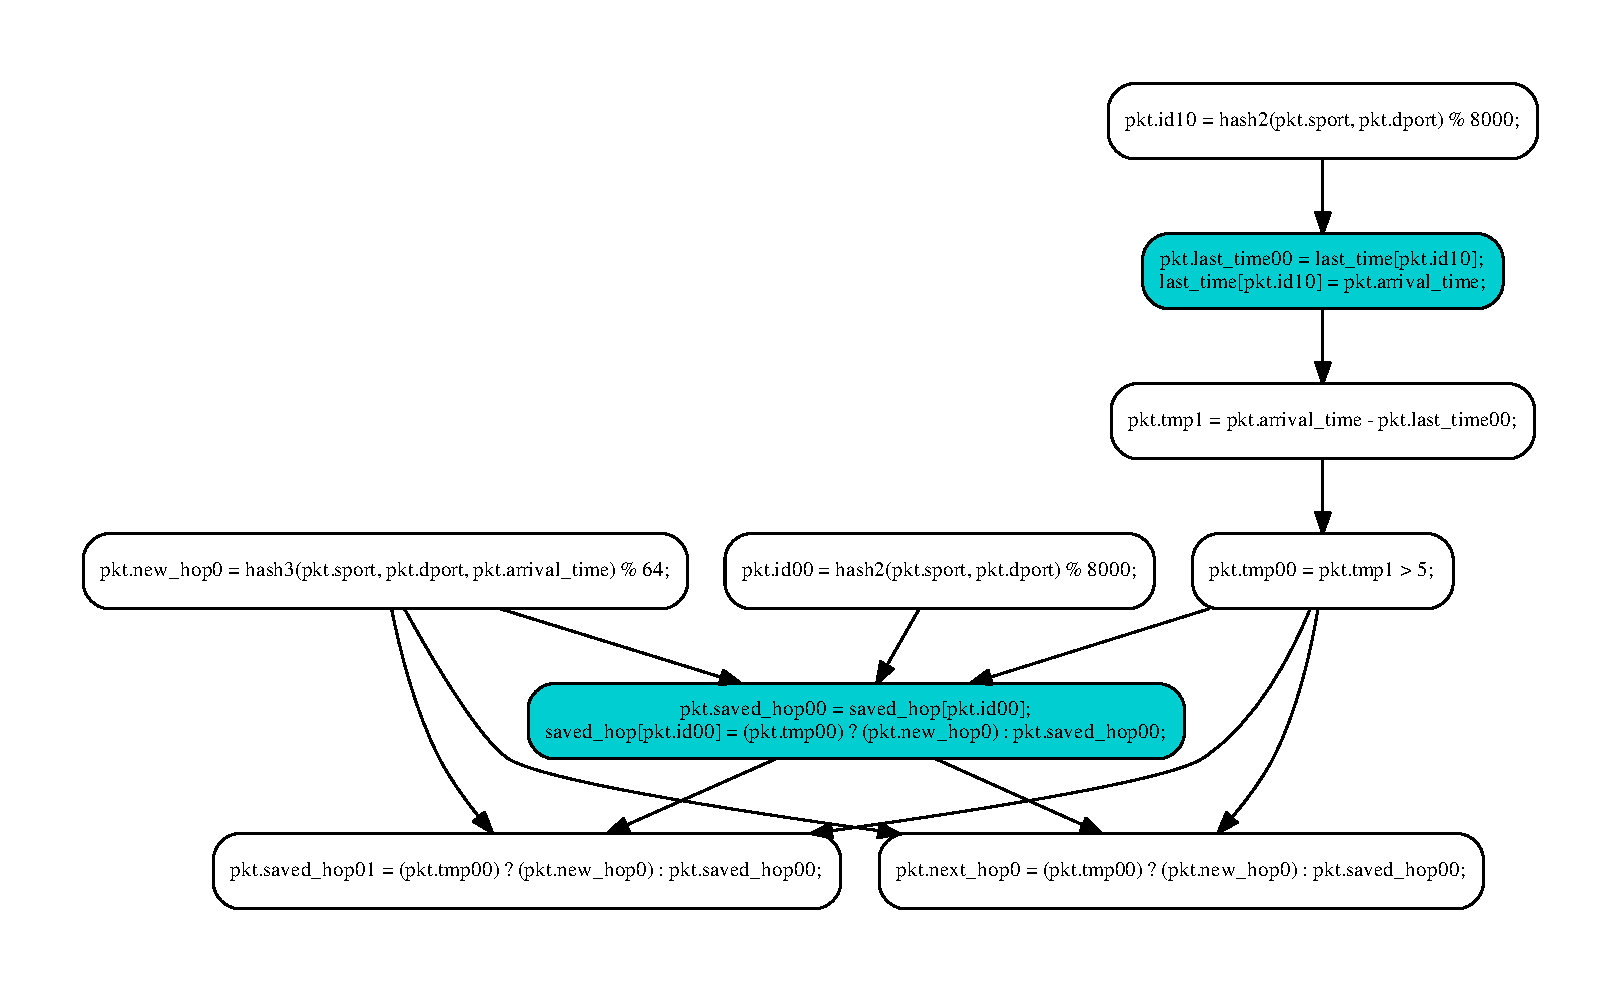
\includegraphics[width=\columnwidth]{dag.pdf}
  \caption{DAG formed by condensing SCCs in Figure~\ref{fig:deps}}
  \label{fig:dag}
\end{figure}
